\documentclass[12pt,letterpaper]{article}
\usepackage{fullpage}
\usepackage[top=2cm, bottom=4.5cm, left=2.5cm, right=2.5cm]{geometry}
\usepackage{amsmath,amsthm,amsfonts,amssymb,amscd}
\usepackage{enumerate}
\usepackage{enumitem}  % You can remove this item if you don't have the enumitem package
\usepackage{fancyhdr}
\usepackage{graphicx}
\usepackage{listings}
\usepackage{hyperref}
\graphicspath{ {./} }
\hypersetup{%
  colorlinks=true,
  linkcolor=blue,
  linkbordercolor={0 0 1}
}
 
\renewcommand\lstlistingname{Algorithm}
\renewcommand\lstlistlistingname{Algorithms}
\def\lstlistingautorefname{Alg.}

\lstdefinestyle{R}{
    language        = R,
    frame           = lines, 
    basicstyle      = \footnotesize,
    keywordstyle    = \color{blue},
    stringstyle     = \color{green},
    commentstyle    = \color{red}\ttfamily
}

\setlength{\parindent}{0.0in}
\setlength{\parskip}{0.05in}

%%%%%%%%%%%%%%%%%%%%%%%%%%%%%%%%%%%%%%%%%%%%%%%%%%%%%%%%%%%%%%%%%%%
% Edit these as appropriate for the header!
%%%%%%%%%%%%%%%%%%%%%%%%%%%%%%%%%%%%%%%%%%%%%%%%%%%%%%%%%%%%%%%%%%%
\newcommand\course{ISyE 8803 HDDA}
\newcommand\hwnumber{1}                           % Homework Number
\newcommand\studentname{Jeff Tilton}         % Name name
\newcommand\username{jtilton6}                  % Username

\chead{\textbf{\Large Homework \hwnumber}}        % You can change
%\chead{\textbf{\Large Midterm Exam}}             % the commented
%\chead{\textbf{\Large Final Exam}}               % lines for exams

%%%%%%%%%%%%%%%%%%%%%%%%%%%%%%%%%%%%%%%%%%%%%%%%%%%%%%%%%%%%%%%%%%%

\pagestyle{fancyplain}
\headheight 35pt
\lhead{\studentname \\ \username}
\rhead{\course \\ \today}
\lfoot{}
\cfoot{}
\rfoot{\small\thepage}
\headsep 1.5em

\begin{document}

\section*{Question 1}

Question 1: The behavior of polynomials fit to data tends to be erratic near the boundaries. The polynomials fit beyond the boundary knots behave even more wildly than the corresponding global polynomials in that region. Assuming the function is linear near the boundaries (where we have less information anyway) is often considered reasonable. A natural quadratic spline adds additional constraints, namely that the function is linear beyond the boundary knots.

 
\begin{align*}
N_1(X)  =& 1,N_{k=1...K-1}(X) = (X-\xi_k)\textsuperscript{2}\textsubscript{+} -(X-\xi_K)\textsuperscript{2}\textsubscript{+}\\
N_2(X)  =& X 
\end{align*}
With constraints:

\begin{align*}
&\beta_3 = 0& \\
&\sum_{k=1}^K \theta_k =0& \\
&\sum_{k=1}^K \xi_K\theta_k =0& \\
\frac{d^2}{dx^2}y(x)=&2\sum_{k=1}^K\theta=0&
\end{align*}


\newpage

\section*{Question 2}

Question 2: 

Let $B_{i,j}(x)$ be the $ith$ B-spline basis function of a uniform quadratic B-spline with 5 knots.  Derive an expression for $B_{0,2}(x)$, $B_{1,2}(x)$, and $B_{2,2}(x)$



\begin{align*}
&B_{i,0}(x)=\begin{cases}
    1, & \text{if $\tau_i\leq x < \tau_{i+1}$}.\\
    0, & \text{otherwise}.
\end{cases}
\\ \\
&B_{0,1}(x)\mbox{ from } [0,1) = x \\
&B_{0,1}(x)\mbox{ from } [1,2) = 2-x \\ \\
%\
&B_{1,1}(x)\mbox{ from } [1,2) = x-1 \\
&B_{1,1}(x)\mbox{ from } [2,3) = 3-x \\ \\
%\
&B_{2,1}(x)\mbox{ from } [2,3) = x-2 \\
&B_{2,1}(x)\mbox{ from } [3,4) = 4-x \\ \\
%\
&B_{3,1}(x)\mbox{ from } [3,4) = x-3 \\
&B_{3,1}(x)\mbox{ from } [4,5) = 5-x \\ \\
%\
&B_{0,2}(x)\mbox{ from } [0,1) = .5x^2 \\
&B_{0,2}(x)\mbox{ from } [1,2) = 3x-x^2-1.5 \\
&B_{0,2}(x)\mbox{ from } [2,3) = .5(3-x)^2 \\ \\
%\ 
&B_{1,2}(x)\mbox{ from } [1,2) = .5(x-1)^2 \\
&B_{1,2}(x)\mbox{ from } [2,3) = .5[(x-1)(3-x)+(4-x)(x-2)] \\
&B_{1,2}(x)\mbox{ from } [3,4) = .5(4-x)^2 \\ \\
%\ 
&B_{2,2}(x)\mbox{ from } [2,3) = .5(x-2)^2 \\
&B_{2,2}(x)\mbox{ from } [3,4) = .5[(x-2)(4-x)+(5-x)(x-3)] \\
&B_{2,2}(x)\mbox{ from } [4,5) = .5(5-x)^2 \\ \\
\end{align*}

\section*{Question 3}
Data provided in this section shows the electrical energy produced by coal in the United States from 1960 to 2018.

\begin{enumerate}[label=\alph*)]



\item Cubic Splines 
Fifteen knots had the lowest mean squared error at 0.49, the resulting curve is seen below.
\begin{center}
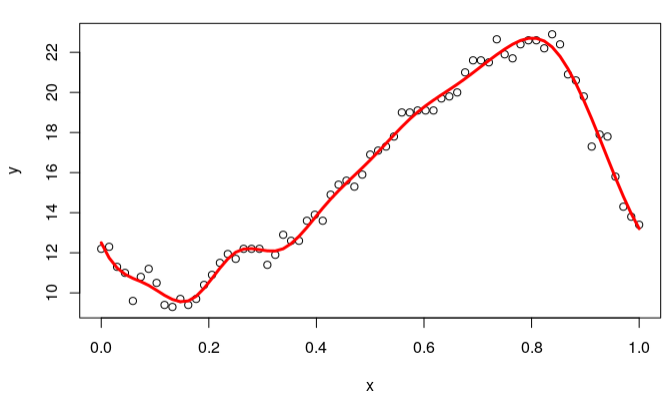
\includegraphics[width=10cm]{cspline.png}
\end{center}
 

\item  B-splines 
Fourteen knots had the lowest mean squared error at 0.18, the resulting curve is seen below.


\begin{center}
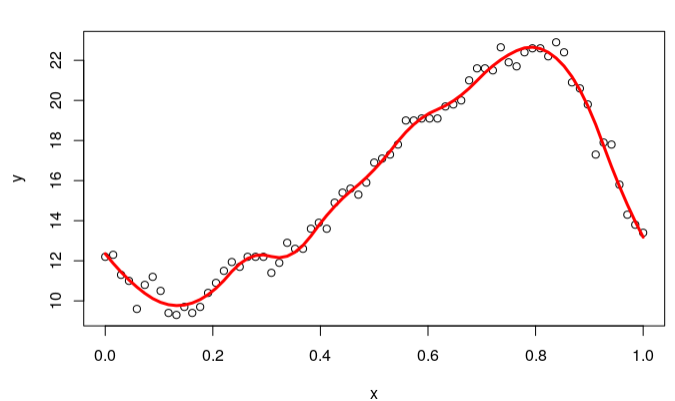
\includegraphics[width=10cm]{bspline.png} 
\end{center}

\item  Smooth Splines 
The lambda with the best mean squared error was 1.23e-05 with a score of 0.28.  The resulting curve is seen below.

\begin{center}
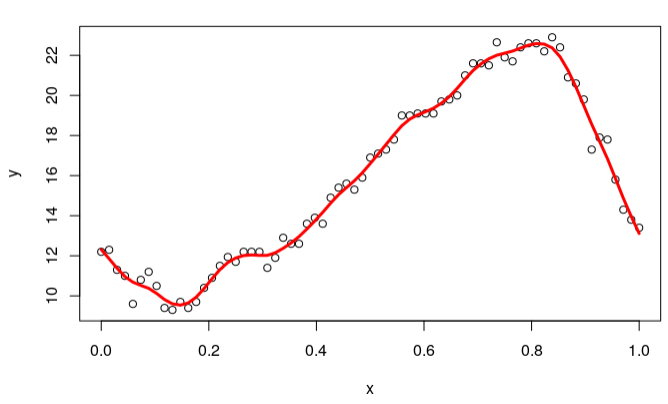
\includegraphics[width=10cm]{sspline.png} 
\end{center}


\item  Kernel regression with Gaussian kernel
The lambda with the best mean squared error was 1 with a score of 0.25.  The resulting curve is seen below.



\begin{center}
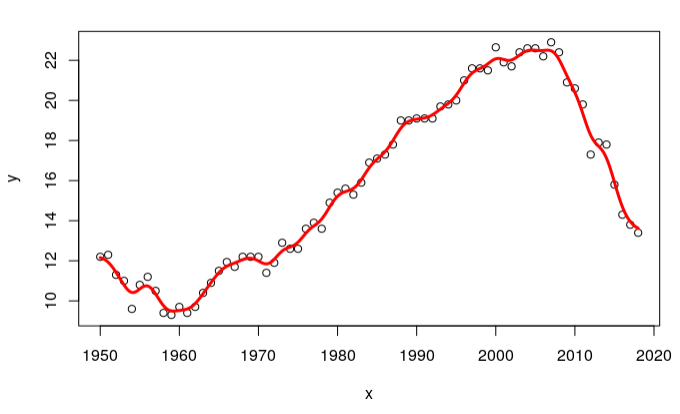
\includegraphics[width=10cm]{kregress.png} 
\end{center}

\end{enumerate}

B-splines produced the curve with the lowest mse.  However, I find the curves almost indistinguishable except for the Kernel Regression that appears to have a little higher bias on the left hand tail compared to the other approaches.



 
\section*{Question 4}

Use B-splines and FPCA to classify the ECG as normal or abnormal. You can use the classification method of your preference.


Random forest was used to classify the B-spline and FPCA coefficients.  Positive classification is defined as correctly identifying an abnormal heart rate.  Data was split between a train and test set, the test set results are shown below.



\begin{enumerate}[label=\alph*)]


\item B-splines

The random forest model with b-spline coefficients had a sensitivity of 0.86, a specificity of 0.91 with results seen in the confusion matrix below.  

\begin{center}
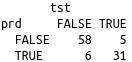
\includegraphics[width=5cm]{conf_bspline.png} 
\end{center}

Where prd is the predicted values and tst are the reference classes.

\item FPCA

The random forest model with b-spline coefficients had a sensitivity of 0.64 and a specificity of 0.94 with results seen in the confusion matrix below.

\begin{center}
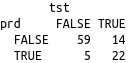
\includegraphics[width=5cm]{conf_fpca.png} 
\end{center}


Where prd is the predicted values and tst are the reference classes.

\end{enumerate}

Classification using the B-splines coefficients results in a better classifier for this problem because it has a much better sensitivity. It is more important to correctly classify an abnormal ECG than correctly classify a normal one and this is shown in th much higher sensitivity score. 

\end{document}
